\section{Preliminaries}
\label{sec:prelim}

This section formalizes the language world model (LWM) studied throughout this work.
We train the world model based on language models using the broad world-knowledge corpora, and unify seven domains under a shared textual representation that enables cross-domain generalization for language world modeling.
We begin by establishing terminology (\S\ref{sec:prelim:terminology}), then present the unified trajectory schema shared across seven domains and training stages (\S\ref{sec:prelim:schema}) and formalize the world modeling objective (\S\ref{sec:prelim:formulation}).

\subsection{Terminology}
\label{sec:prelim:terminology}

We use the following terms consistently throughout this report.
\textbf{LWM training} refers to training the world model itself through three stages: continual pre-training (\textbf{LWM CPT}, \S\ref{sec:pipeline:cpt}), supervised fine-tuning (\textbf{LWM SFT}, \S\ref{sec:pipeline:sft}), and reinforcement learning (\textbf{LWM RL}, \S\ref{sec:pipeline:rl}).
Separately, \textbf{Sim~RL} trains a policy agent via RL using a LWM as an environment simulator (\S\ref{sec:app:simulator}), while \textbf{Real~RL} trains the same agent against a live, real-world environment (e.g., an actual search engine or a running terminal).

Throughout this report, \textbf{trajectory} refers to an \textbf{environment trajectory}, which is structurally a multi-turn dialogue between the agent and the environment, represented as a sequence of (action, observation) pairs.
In contrast, an \textbf{agentic trajectory} is the agent's single completion for a task, a multi-step tool-integrated reasoning trace that interleaves the agent's internal thinking and action selection with the environment's observations.
Environment trajectories can be extracted from agentic trajectories by stripping agent reasoning and retaining only (action, observation) pairs, or collected directly from raw interaction logs.


\begin{figure*}[t]
\centering
\begin{tcolorbox}[
  colback=gray!3, colframe=black!50, boxrule=0.5pt,
  title={\small System Prompt --- Terminal LWM RL},
  fonttitle=\bfseries\small,
  left=4pt, right=4pt, top=2pt, bottom=2pt
]
\scriptsize
\textbf{\color{blue!70!black}[1] Task Description} \hfill \textit{static}\\[2pt]
You are a \textbf{Terminal World Model} --- a precise terminal state simulator. Your task is to predict the exact output of a Linux/Unix terminal after executing a given command or sequence of commands. Your goal is to be as faithful as possible to real terminal behavior while maintaining consistency and logical correctness across the interaction sequence.\\[1pt]
\textit{Given:} (1)~Historical Context (optional); (2)~Current Terminal State; (3)~User Action (keystrokes).\\\textit{Predict:} the exact next terminal state after all actions are executed.\\[1pt]
Core Responsibilities: State Prediction~$\mid$~Context Maintenance~$\mid$~Behavioral Fidelity\\[1pt]
{\color{gray}\textit{[\,\dots\; state transition rules, side-effect tracking, error handling, output formatting \dots\,]}}

\tcbline

\textbf{\color{blue!70!black}[2] Action Space} \hfill \textit{static}\\[2pt]
User actions are JSON arrays of command objects:~~{\ttfamily\char`\{``keystrokes'': ``ls -la\char`\\n'', ``duration'': 0.1\char`\}}\\[1pt]
Keystrokes: {\ttfamily\char`\\n} = execute;~~{\ttfamily C-c} = SIGINT;~~{\ttfamily C-d} = EOF;~~{\ttfamily C-z} = SIGTSTP;~~{\ttfamily C-l} = clear screen\\[1pt]
Shell constructs: pipes, redirects, command chaining;~~Programs: shell builtins, editors (vim/nano), REPLs, pagers

\tcbline

\textbf{\color{red!70!black}[3] Initial State} \hfill \textit{dynamic, injected per trajectory}\\[2pt]
The initial container snapshot of the terminal environment is:\\[1pt]
OS: Ubuntu 22.04.3 LTS (x86\_64)\quad Kernel: Linux 5.15.0-134-generic\\
Packages: Python 3.10.12, pip 23.2.1, Node 18.17.1, gcc 11.4.0, git 2.34.1, Docker 24.0.5\\
Disk: 64\,GB (41\,GB free)\quad RAM: 16\,GB\quad Working dir: {\ttfamily /workspace}\\[1pt]
The initial terminal state is:\\[1pt]
{\ttfamily root@6b254155-5503-4b86-837b-fd0f080ab297:/workspace\char`\#}

\tcbline

\textbf{\color{blue!70!black}[4] Demonstrations} \hfill \textit{static}\\[2pt]
\textbf{Turn~1} \,\textbar\, Action: {\ttfamily\dq{}git clone https://github.com/expressjs/express.git /tmp/express\char`\\n\dq{}}\\
\hphantom{\textbf{Turn~1} \,\textbar\,} Observation: {\ttfamily root@6b254155:/workspace\char`\# git clone https://github.com/expressjs/express.git /tmp/express}\\
\hphantom{\textbf{Turn~1} \,\textbar\, Observation: }{\ttfamily Cloning into \sq{}/tmp/express\sq{}...}\\[1pt]
\textbf{Turn~2} \,\textbar\, Action: {\ttfamily\dq{}\dq{}}, duration=3.0\\
\hphantom{\textbf{Turn~2} \,\textbar\,} Observation: {\ttfamily remote: Enumerating objects: 32841, done.}\\
\hphantom{\textbf{Turn~2} \,\textbar\, Observation: }{\ttfamily remote: Counting objects: 100\char`\% (1205/1205), done.}\\
\hphantom{\textbf{Turn~2} \,\textbar\, Observation: }{\ttfamily Receiving objects: 100\char`\% (32841/32841), 12.76 MiB | 8.53 MiB/s, done.}\\
\hphantom{\textbf{Turn~2} \,\textbar\, Observation: }{\ttfamily Resolving deltas: 100\char`\% (21567/21567), done.}\\
\hphantom{\textbf{Turn~2} \,\textbar\, Observation: }{\ttfamily root@6b254155:/workspace\char`\#}\\[1pt]
{\color{gray}\textit{[\,\dots\; 6 more turns demonstrating directory navigation and build operations \dots\,]}}

\tcbline

\textbf{\color{red!70!black}[5] Simulation Instruction} \hfill \textit{dynamic, injected per trajectory}\\[2pt]
Simulate a system with CUDA~11.8 drivers and only 2\,GB free disk space. {\ttfamily pip install torch==2.1.0} should complete the download phase normally (progress bar reaching 100\char`\%), then fail during unpacking of {\ttfamily libtorch\_cuda.so} with {\ttfamily OSError: [Errno 28] No space left on device}. After the failure, {\ttfamily pip cache list} should report the partially downloaded {\ttfamily .whl} file still present. {\ttfamily df -h} should show {\ttfamily /tmp} at 100\char`\% usage.\\[1pt]
{\color{gray}\textit{See \S\ref{sec:app:controllable} for the controllable simulation capability.}}
\end{tcolorbox}
\caption{
Anatomy of a Terminal domain LWM RL system prompt, showing the five components defined in \S\ref{sec:prelim:schema}. {\color{blue!70!black}Blue} = static (shared across trajectories); {\color{red!70!black}red} = dynamic (injected per trajectory).
}
\label{fig:system_prompt_example}
\end{figure*}


\subsection{Unified Environment Trajectory Schema}
\label{sec:prelim:schema}

Training a single world model across seven domains with state representations as varied as file-system snapshots for Terminal and UI view hierarchies for Android requires a shared format.
We adopt the following environment trajectory schema uniformly across all seven domains and training stages:

\begin{tcolorbox}[
  colback=gray!3, colframe=black!50,
  boxrule=0.5pt, arc=2pt,
  title={\small\bfseries Unified Environment Trajectory Schema},
  top=4pt, bottom=4pt, left=6pt, right=6pt
]
\small
\begin{tabular}{@{}r@{$\;\,:=\;\,$}l@{}}
$\mathrm{system\_prompt}$ & $\mathrm{task\_description} \oplus \mathrm{action\_space} \oplus \mathrm{initial\_state} \oplus \mathrm{demonstrations} \oplus \mathrm{simulation\_instruction}$ \\[4pt]
$\mathrm{turn}_t$ & $(\mathrm{action}_t,\,\mathrm{observation}_t)$ \\[4pt]
$\mathrm{trajectory}$ & $\mathrm{system\_prompt} \oplus [\mathrm{turn}_1, \ldots, \mathrm{turn}_T]$
\end{tabular}
\end{tcolorbox}

In this schema, an \emph{action} is the agent's output at one turn (e.g., a tool call or shell command) and an \emph{observation} is the environment's feedback (e.g., tool response or command output).

Figure~\ref{fig:system_prompt_example} illustrates a fully assembled system prompt from the Terminal domain, with representative excerpts from each component.
The system prompt has five components, whose construction is detailed in \S\ref{sec:pipeline:prompt}.
The \emph{task description} instructs the model to act as a world model for a specific domain and defines the simulation objective.
The \emph{action space} enumerates the available tools or operations and their calling conventions.
The \emph{initial state} specifies the environment's starting configuration before any interaction begins: installed packages, file-system layout, UI screen state, or any other precondition that the trajectory assumes.
Together with the interaction history and current action, a sufficiently detailed initial state substantially constrains the expected observation.
\emph{Demonstrations} are optional few-shot (action, observation) examples.
The \emph{simulation instruction} specifies controllable simulation conditions (e.g., ``hide the answer from the \texttt{web\_search} responses'') and is used primarily for the controllable simulation experiments (\S\ref{sec:app:controllable}).


\begin{figure*}[t]
\centering
\begin{subfigure}[t]{\linewidth}
  \centering
  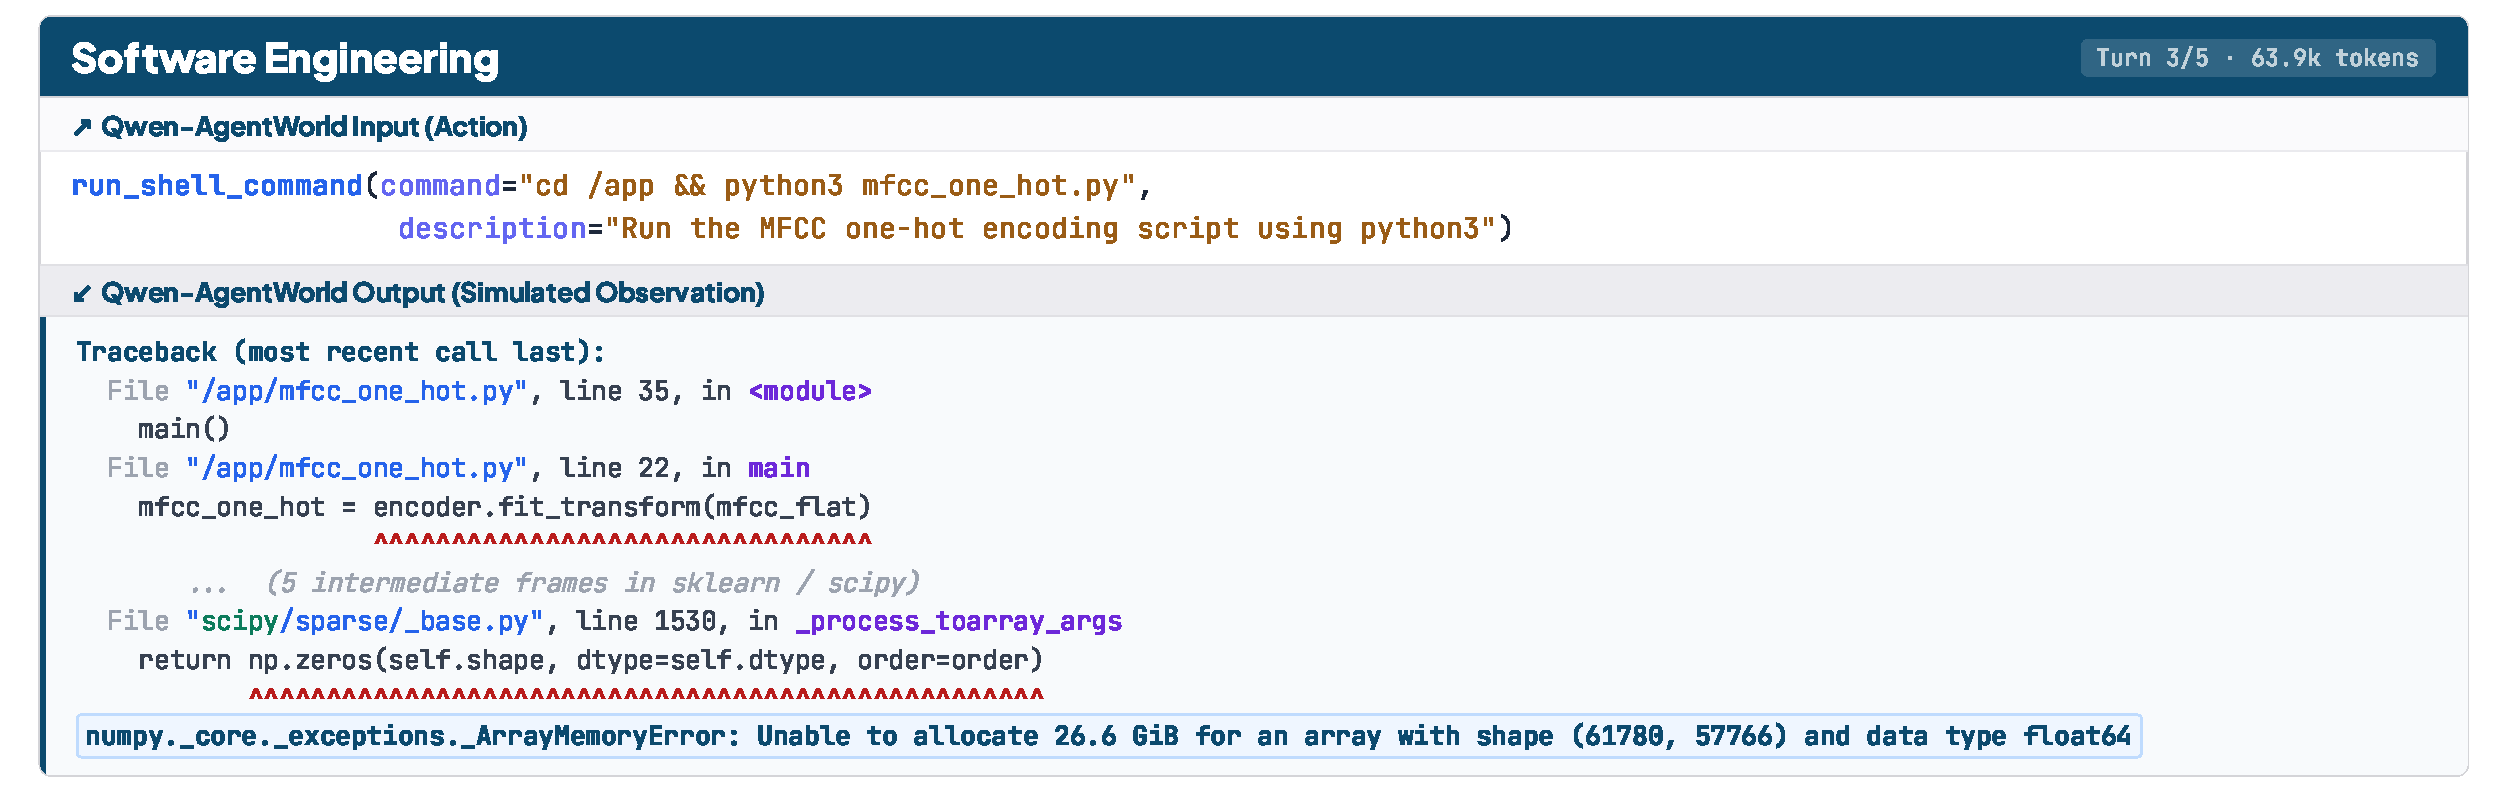
\includegraphics[width=\linewidth]{figures/fig_swe.pdf}
  \caption{
  \textbf{SWE} (text-based): The agent runs a Python script; the world model predicts the full traceback including an out-of-memory error during one-hot encoding.
  }
  \label{fig:domain_example_swe}
\end{subfigure}
\vspace{4pt}
\begin{subfigure}[t]{\linewidth}
  \centering
  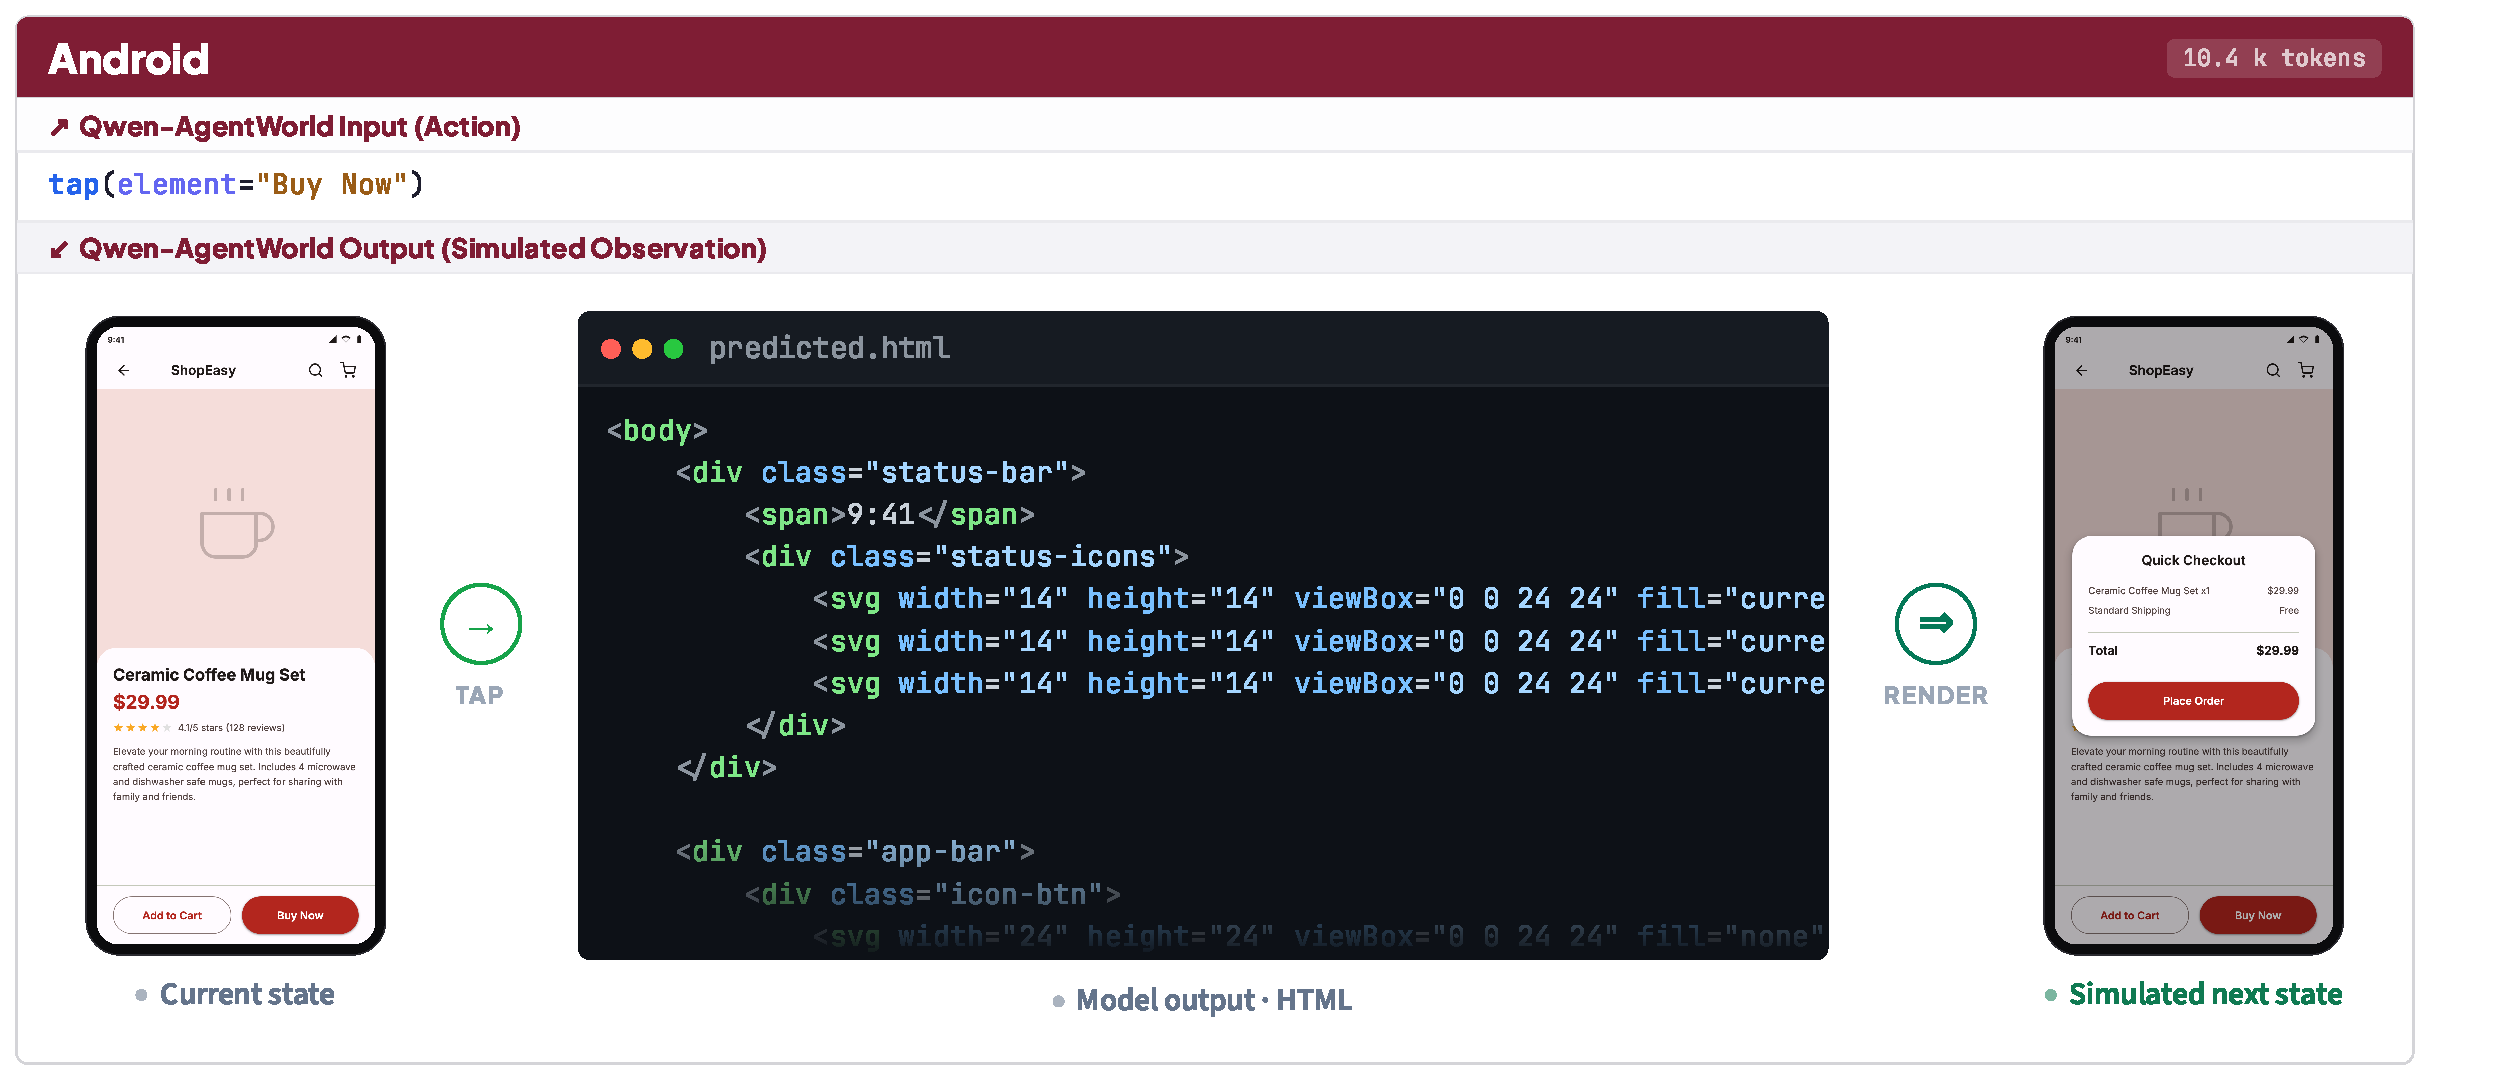
\includegraphics[width=\linewidth]{figures/fig_android.pdf}
  \caption{
  \textbf{Android} (GUI): The agent taps ``Buy Now'' on a product page; the world model predicts an HTML representation of the next screen, which is rendered as the predicted checkout sheet.
  }
  \label{fig:domain_example_android}
\end{subfigure}
\caption{Representative interaction examples from a text-based domain (SWE) and a GUI domain (Android), illustrating the breadth of the observation space.}
\label{fig:domain_examples}
\end{figure*}



\subsection{Language World Model}
\label{sec:prelim:formulation}

A language world model (LWM) is a conditional text generator that predicts the next environment observation given the interaction history and the agent's current action.
Let $c$ denote the system prompt, $o_t$ the environment observation at turn $t$, and $a_t$ the agent's action. The LWM $f_\theta$ produces:
\begin{equation}
    \hat{o}_{t+1} = f_\theta(c,\, o_{\leq t},\, a_{\leq t}),
\end{equation}
where the conditioning context comprises $c$, the full interaction history, and the current action. The training target is the ground-truth observation $o_{t+1}$.

Table~\ref{tab:domain_taxonomy} lists all seven domains with their observation and action representations.
In \emph{stateless} environments (e.g., Search), state is carried implicitly in the conversation history, whereas \emph{stateful} environments (e.g., Terminal, OS) maintain an explicit internal state that evolves with each action.
In both cases the LWM operates over the same observation sequence, as formalized by the schema in \S\ref{sec:prelim:schema}.
Yet the diversity of domains ensures that a single world-modeling objective simultaneously exercises reasoning, knowledge, and long-context understanding.
These capabilities are also foundational to general agents (\S\ref{sec:app:foundation}).

\clearpage

\begin{table}[!ht]
\caption{The seven domains covered by \method, with their action, observation, and core capability exercised by next-state prediction.}
\label{tab:domain_taxonomy}
\centering
\small
\resizebox{\linewidth}{!}{%
\begin{tabular}{@{}llll@{}}
\toprule
\textbf{Domain} & \textbf{Action} & \textbf{Observation} & \textbf{Core Capability} \\
\midrule
MCP      & JSON Tool Call               & Tool response (file content, DB, etc.) & Factual world knowledge \\
Search   & Web Search / Web Extractor   & Conversation history (query + results) & Factual world knowledge \\
SWE      & Read / Edit / Bash / \ldots  & Tool output (file content + diffs) & Code execution reasoning \\
Terminal & Bash Commands / Keystrokes   & Terminal output (stdout + shell prompt) & Long-context causal reasoning \\
Android  & Touch / Swipe / Type / ...         & UI view hierarchy + app state & Visual state reasoning \\
Web      & Click / Type / Navigate / ...     & Accessibility tree + browser state & Visual state reasoning \\
OS       & Mouse / Keyboard             & Accessibility tree + window/app state & Visual state reasoning \\
\bottomrule
\end{tabular}
}
\end{table}

Figure~\ref{fig:domain_examples} illustrates this breadth with one representative example from each category.
In SWE (Figure~\ref{fig:domain_example_swe}), the agent runs a Python script and the LWM must reason through memory allocation and array dimensions to predict the resulting out-of-memory traceback.
In Android (Figure~\ref{fig:domain_example_android}), the agent taps a UI element, and the LWM must infer how the interaction transforms the page layout and predict the resulting screen as renderable HTML.
Appendix~\ref{sec:appendix:domain_examples} presents interaction examples for other domains.

